% -*- compile-command: "cd .. && make" -*-
\documentclass[document.tex]{subfiles}
\begin{document}

\chapter{Platform}
\label {ch:platform}

\todo {Describe the components that were extracted (i.e. what the extracted libraries do, what additional functionality we've added), and link to the sections discussing their design. There should be one section per component, plus an overview section showing the package diagram of the sections are related. The last section will discuss unit testing, and the use of the case studies as integration testing to ensure that new package versions continue working with each other}.

\sectionnote {BM}
\section {Overview}

\todo {Add an introduction here}

The platform consists of both third-party packages and new utility packages that leverage them. A package diagram illustrating the relationships between the packages that make up the platform is given in Figure \ref{fig:platform-package-diagram}.

In particular, Devise and Pundit were selected to provide authentication and authorization, AASM was also selected to provide a domain-specific language for workflow modeling. All of these third-party packages are actively maintained and were applied in building the fourth-year project system without encountering any defects or design flaws that interfered with implementation. Stonepath itself is omitted from the platform; in the prototype and case study, it was determined that aside from AASM, its features did not improve developer productivity. \todo {Add a conclusion section to the case study to support this.}

Four new utility libraries were developed on top of the selected third-party libraries. These libraries are described in detail in the following sections.

\begin{figure}[!ht]
\centering 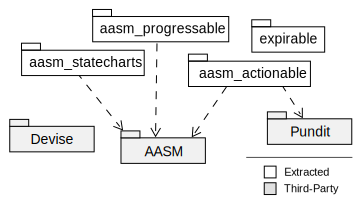
\includegraphics[width=4.5in]{./img/platform/platform-package-diagram}
\caption{Package diagram of the new workflow platform.}
\label{fig:platform-package-diagram}
\end{figure}

\FloatBarrier


\sectionnote {BM}
\section {expirable}


\sectionnote {BM}
\section {aasm\_statecharts}

Although AASM provides a domain specific language that is more readable and maintainable than implementing the state machine pattern, it's event-oriented approach makes it difficult to determine which events are possible in which state. Additionally, it is difficult understand a workflow encoded in AASM without reading the entire specification, even if a developer only wants to get a general sense of the flow of events. Thus, it seems useful to be able to convert back from AASM definitions to diagrams of state machines.

While several tools exist to general state machine diagrams from AASM definitions, these tools fail to capture the full range of concepts expressed by AASM. All of the existing tools, such as RailRoad \cite{railroad}, can generate finite state machine diagrams from AASM descriptions, but the generated diagrams lack guards, actions, or other features of extended state machines or statecharts.

\verb!aasm_statecharts! is a new utility designed to address these shortcomings. It performs a mapping from AASM metadata extracted from Rails models to Graphviz \cite{graphviz} definitions, by converting each state to a styled Graphviz node and each event to a edge. It extracts named guards and actions (i.e. those encoded in the form \verb!on_transition: :action_name! instead of \verb!on_transition: Proc.new { ... }!) from the metadata, though it has no way of handling anonymous actions.

\todo {Distinguish named vs. anonymous callbacks when AASM is introduced.}

\verb!aasm_statecharts! is available at \url{https://github.com/WorkflowsOnRails/aasm_statecharts}, or it may be installed from the \verb!aasm_statecharts! gem.
A short manual is available on the project's GitHub page, and is also attached to this report in section \ref{sec:aasm-statecharts-manual} in Appendix \ref{ch:appendix-manuals}.

\todo {Briefly discuss testing}

\sectionnote {BM}
\section {aasm\_progressable}


\sectionnote {BM}
\section {aasm\_actionable}


\sectionnote {BM}
\section {Missing Functionality}



\end{document}
